\documentclass[14pt]{extbook}
\usepackage{multicol, enumerate, enumitem, hyperref, color, soul, setspace, parskip, fancyhdr} %General Packages
\usepackage{amssymb, amsthm, amsmath, latexsym, units, mathtools} %Math Packages
\everymath{\displaystyle} %All math in Display Style
% Packages with additional options
\usepackage[headsep=0.5cm,headheight=12pt, left=1 in,right= 1 in,top= 1 in,bottom= 1 in]{geometry}
\usepackage[usenames,dvipsnames]{xcolor}
\usepackage{dashrule}  % Package to use the command below to create lines between items
\newcommand{\litem}[1]{\item#1\hspace*{-1cm}\rule{\textwidth}{0.4pt}}
\pagestyle{fancy}
\lhead{Progress Quiz 8}
\chead{}
\rhead{Version ALL}
\lfoot{5493-4176}
\cfoot{}
\rfoot{Summer C 2021}
\begin{document}

\begin{enumerate}
\litem{
Construct the lowest-degree polynomial given the zeros below. Then, choose the intervals that contain the coefficients of the polynomial in the form $ax^3+bx^2+cx+d$.\[ \frac{-4}{3}, \frac{4}{5}, \text{ and } \frac{6}{5} \]\begin{enumerate}[label=\Alph*.]
\item \( a \in [70, 77], b \in [-53, -41], c \in [-130, -119], \text{ and } d \in [86, 98] \)
\item \( a \in [70, 77], b \in [50, 55], c \in [-130, -119], \text{ and } d \in [-100, -88] \)
\item \( a \in [70, 77], b \in [-53, -41], c \in [-130, -119], \text{ and } d \in [-100, -88] \)
\item \( a \in [70, 77], b \in [-251, -249], c \in [271, 273], \text{ and } d \in [-100, -88] \)
\item \( a \in [70, 77], b \in [-131, -126], c \in [-33, -27], \text{ and } d \in [86, 98] \)

\end{enumerate} }
\litem{
Describe the end behavior of the polynomial below.\[ f(x) = 5(x - 7)^{4}(x + 7)^{5}(x - 4)^{3}(x + 4)^{3} \]\begin{enumerate}[label=\Alph*.]
\begin{multicols}{2}\item 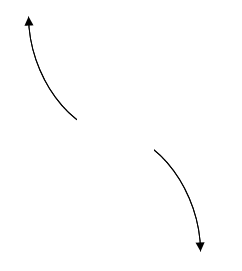
\includegraphics[width = 0.3\textwidth]{../Figures/polyEndBehaviorCopyAA.png}\item 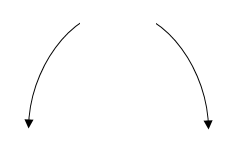
\includegraphics[width = 0.3\textwidth]{../Figures/polyEndBehaviorCopyBA.png}\item 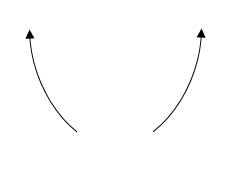
\includegraphics[width = 0.3\textwidth]{../Figures/polyEndBehaviorCopyCA.png}\item 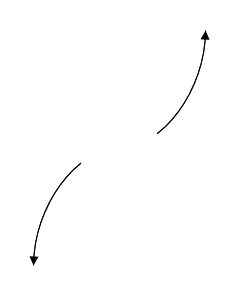
\includegraphics[width = 0.3\textwidth]{../Figures/polyEndBehaviorCopyDA.png}\end{multicols}\item None of the above.
\end{enumerate} }
\litem{
Construct the lowest-degree polynomial given the zeros below. Then, choose the intervals that contain the coefficients of the polynomial in the form $x^3+bx^2+cx+d$.\[ -2 + 4 i \text{ and } 1 \]\begin{enumerate}[label=\Alph*.]
\item \( b \in [0.7, 1.4], c \in [-6, -3], \text{ and } d \in [2, 11] \)
\item \( b \in [0.7, 1.4], c \in [-1, 5], \text{ and } d \in [-9, 0] \)
\item \( b \in [-6.9, -1.6], c \in [14, 23], \text{ and } d \in [13, 26] \)
\item \( b \in [1.6, 6.2], c \in [14, 23], \text{ and } d \in [-25, -14] \)
\item \( \text{None of the above.} \)

\end{enumerate} }
\litem{
Describe the end behavior of the polynomial below.\[ f(x) = -4(x - 4)^{5}(x + 4)^{10}(x + 6)^{3}(x - 6)^{5} \]\begin{enumerate}[label=\Alph*.]
\begin{multicols}{2}\item 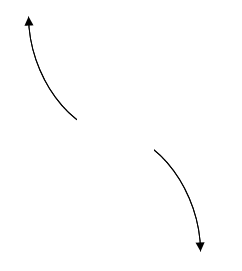
\includegraphics[width = 0.3\textwidth]{../Figures/polyEndBehaviorAA.png}\item 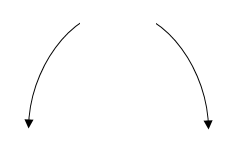
\includegraphics[width = 0.3\textwidth]{../Figures/polyEndBehaviorBA.png}\item 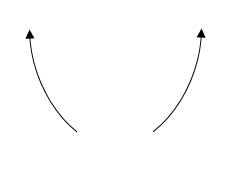
\includegraphics[width = 0.3\textwidth]{../Figures/polyEndBehaviorCA.png}\item 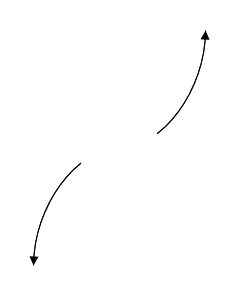
\includegraphics[width = 0.3\textwidth]{../Figures/polyEndBehaviorDA.png}\end{multicols}\item None of the above.
\end{enumerate} }
\litem{
Which of the following equations \textit{could} be of the graph presented below?
\begin{center}
    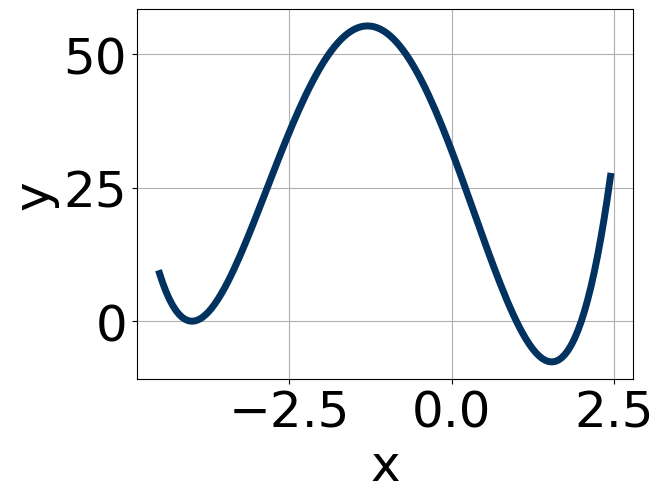
\includegraphics[width=0.5\textwidth]{../Figures/polyGraphToFunctionCopyA.png}
\end{center}
\begin{enumerate}[label=\Alph*.]
\item \( 10(x + 4)^{6} (x - 1)^{11} (x - 2)^{5} \)
\item \( 10(x + 4)^{8} (x - 1)^{10} (x - 2)^{5} \)
\item \( -12(x + 4)^{4} (x - 1)^{5} (x - 2)^{8} \)
\item \( -6(x + 4)^{10} (x - 1)^{11} (x - 2)^{11} \)
\item \( 17(x + 4)^{7} (x - 1)^{10} (x - 2)^{5} \)

\end{enumerate} }
\litem{
Describe the zero behavior of the zero $x = -5$ of the polynomial below.\[ f(x) = -9(x - 5)^{2}(x + 5)^{7}(x + 7)^{8}(x - 7)^{10} \]\begin{enumerate}[label=\Alph*.]
\begin{multicols}{2}\item 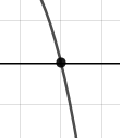
\includegraphics[width = 0.3\textwidth]{../Figures/polyZeroBehaviorAA.png}\item 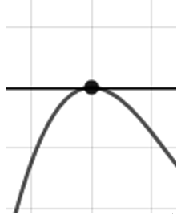
\includegraphics[width = 0.3\textwidth]{../Figures/polyZeroBehaviorBA.png}\item 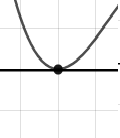
\includegraphics[width = 0.3\textwidth]{../Figures/polyZeroBehaviorCA.png}\item 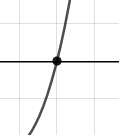
\includegraphics[width = 0.3\textwidth]{../Figures/polyZeroBehaviorDA.png}\end{multicols}\item None of the above.
\end{enumerate} }
\litem{
Construct the lowest-degree polynomial given the zeros below. Then, choose the intervals that contain the coefficients of the polynomial in the form $x^3+bx^2+cx+d$.\[ -2 - 3 i \text{ and } 2 \]\begin{enumerate}[label=\Alph*.]
\item \( b \in [-2.71, -1.5], c \in [3.3, 9.2], \text{ and } d \in [22.8, 26.7] \)
\item \( b \in [1.42, 2.12], c \in [3.3, 9.2], \text{ and } d \in [-26.6, -24.8] \)
\item \( b \in [0.14, 1.15], c \in [0.2, 1.1], \text{ and } d \in [-7.3, -4.4] \)
\item \( b \in [0.14, 1.15], c \in [-3.6, 0.6], \text{ and } d \in [-4.4, -1.3] \)
\item \( \text{None of the above.} \)

\end{enumerate} }
\litem{
Construct the lowest-degree polynomial given the zeros below. Then, choose the intervals that contain the coefficients of the polynomial in the form $ax^3+bx^2+cx+d$.\[ \frac{-1}{4}, 7, \text{ and } \frac{7}{5} \]\begin{enumerate}[label=\Alph*.]
\item \( a \in [18, 22], b \in [-170, -159], c \in [152, 163], \text{ and } d \in [42, 51] \)
\item \( a \in [18, 22], b \in [106, 113], c \in [-227, -221], \text{ and } d \in [42, 51] \)
\item \( a \in [18, 22], b \in [-178, -171], c \in [231, 239], \text{ and } d \in [-53, -47] \)
\item \( a \in [18, 22], b \in [159, 164], c \in [152, 163], \text{ and } d \in [-53, -47] \)
\item \( a \in [18, 22], b \in [-170, -159], c \in [152, 163], \text{ and } d \in [-53, -47] \)

\end{enumerate} }
\litem{
Which of the following equations \textit{could} be of the graph presented below?
\begin{center}
    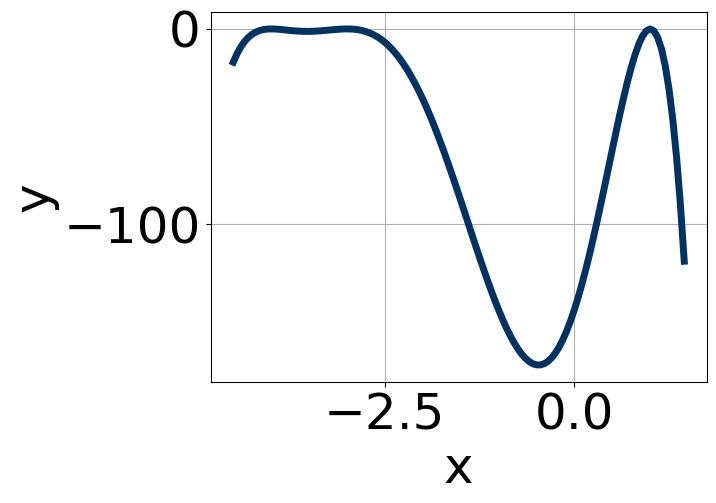
\includegraphics[width=0.5\textwidth]{../Figures/polyGraphToFunctionA.png}
\end{center}
\begin{enumerate}[label=\Alph*.]
\item \( -20(x + 4)^{10} (x + 3)^{5} (x - 1)^{7} \)
\item \( 9(x + 4)^{8} (x + 3)^{8} (x - 1)^{9} \)
\item \( 10(x + 4)^{4} (x + 3)^{10} (x - 1)^{6} \)
\item \( -3(x + 4)^{6} (x + 3)^{6} (x - 1)^{8} \)
\item \( -16(x + 4)^{6} (x + 3)^{4} (x - 1)^{5} \)

\end{enumerate} }
\litem{
Describe the zero behavior of the zero $x = 7$ of the polynomial below.\[ f(x) = -7(x + 7)^{5}(x - 7)^{10}(x - 4)^{4}(x + 4)^{7} \]\begin{enumerate}[label=\Alph*.]
\begin{multicols}{2}\item 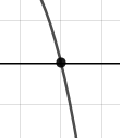
\includegraphics[width = 0.3\textwidth]{../Figures/polyZeroBehaviorCopyAA.png}\item 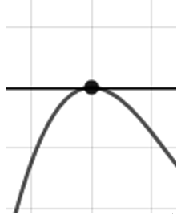
\includegraphics[width = 0.3\textwidth]{../Figures/polyZeroBehaviorCopyBA.png}\item 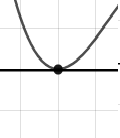
\includegraphics[width = 0.3\textwidth]{../Figures/polyZeroBehaviorCopyCA.png}\item 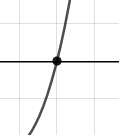
\includegraphics[width = 0.3\textwidth]{../Figures/polyZeroBehaviorCopyDA.png}\end{multicols}\item None of the above.
\end{enumerate} }
\litem{
Construct the lowest-degree polynomial given the zeros below. Then, choose the intervals that contain the coefficients of the polynomial in the form $ax^3+bx^2+cx+d$.\[ \frac{-7}{4}, -1, \text{ and } -3 \]\begin{enumerate}[label=\Alph*.]
\item \( a \in [2, 5], b \in [21, 29], c \in [37, 41], \text{ and } d \in [-23, -18] \)
\item \( a \in [2, 5], b \in [21, 29], c \in [37, 41], \text{ and } d \in [20, 22] \)
\item \( a \in [2, 5], b \in [-24, -16], c \in [37, 41], \text{ and } d \in [-23, -18] \)
\item \( a \in [2, 5], b \in [6, 12], c \in [-19, -11], \text{ and } d \in [-23, -18] \)
\item \( a \in [2, 5], b \in [0, 3], c \in [-33, -25], \text{ and } d \in [20, 22] \)

\end{enumerate} }
\litem{
Describe the end behavior of the polynomial below.\[ f(x) = 5(x + 4)^{2}(x - 4)^{3}(x + 8)^{5}(x - 8)^{6} \]\begin{enumerate}[label=\Alph*.]
\begin{multicols}{2}\item 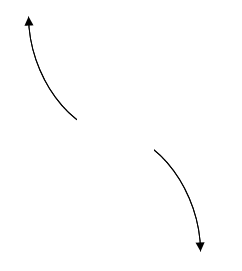
\includegraphics[width = 0.3\textwidth]{../Figures/polyEndBehaviorCopyAB.png}\item 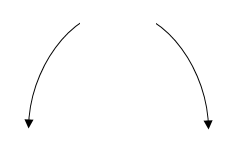
\includegraphics[width = 0.3\textwidth]{../Figures/polyEndBehaviorCopyBB.png}\item 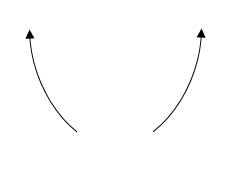
\includegraphics[width = 0.3\textwidth]{../Figures/polyEndBehaviorCopyCB.png}\item 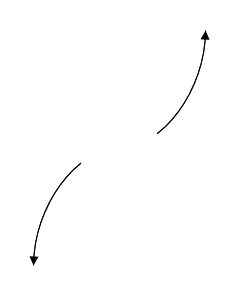
\includegraphics[width = 0.3\textwidth]{../Figures/polyEndBehaviorCopyDB.png}\end{multicols}\item None of the above.
\end{enumerate} }
\litem{
Construct the lowest-degree polynomial given the zeros below. Then, choose the intervals that contain the coefficients of the polynomial in the form $x^3+bx^2+cx+d$.\[ 4 - 5 i \text{ and } 4 \]\begin{enumerate}[label=\Alph*.]
\item \( b \in [-13, -11], c \in [71, 74], \text{ and } d \in [-171, -156] \)
\item \( b \in [9, 15], c \in [71, 74], \text{ and } d \in [156, 167] \)
\item \( b \in [-6, 2], c \in [-11, -2], \text{ and } d \in [16, 20] \)
\item \( b \in [-6, 2], c \in [-1, 11], \text{ and } d \in [-28, -19] \)
\item \( \text{None of the above.} \)

\end{enumerate} }
\litem{
Describe the end behavior of the polynomial below.\[ f(x) = -2(x + 7)^{3}(x - 7)^{4}(x - 8)^{3}(x + 8)^{5} \]\begin{enumerate}[label=\Alph*.]
\begin{multicols}{2}\item 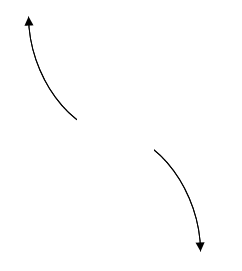
\includegraphics[width = 0.3\textwidth]{../Figures/polyEndBehaviorAB.png}\item 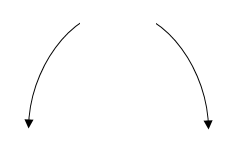
\includegraphics[width = 0.3\textwidth]{../Figures/polyEndBehaviorBB.png}\item 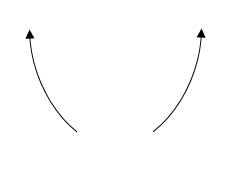
\includegraphics[width = 0.3\textwidth]{../Figures/polyEndBehaviorCB.png}\item 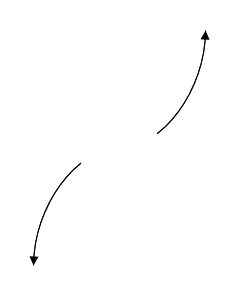
\includegraphics[width = 0.3\textwidth]{../Figures/polyEndBehaviorDB.png}\end{multicols}\item None of the above.
\end{enumerate} }
\litem{
Which of the following equations \textit{could} be of the graph presented below?
\begin{center}
    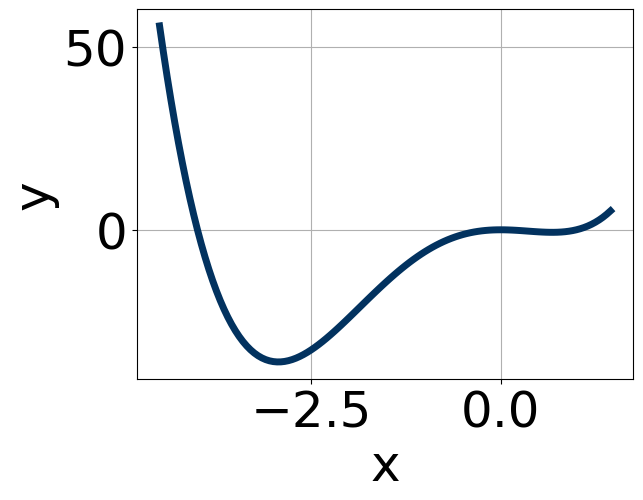
\includegraphics[width=0.5\textwidth]{../Figures/polyGraphToFunctionCopyB.png}
\end{center}
\begin{enumerate}[label=\Alph*.]
\item \( -7x^{10} (x - 1)^{9} (x + 4)^{8} \)
\item \( 16x^{10} (x - 1)^{5} (x + 4)^{9} \)
\item \( -12x^{8} (x - 1)^{9} (x + 4)^{9} \)
\item \( 13x^{10} (x - 1)^{8} (x + 4)^{11} \)
\item \( 4x^{5} (x - 1)^{6} (x + 4)^{9} \)

\end{enumerate} }
\litem{
Describe the zero behavior of the zero $x = -7$ of the polynomial below.\[ f(x) = -5(x - 2)^{6}(x + 2)^{4}(x + 7)^{6}(x - 7)^{5} \]\begin{enumerate}[label=\Alph*.]
\begin{multicols}{2}\item 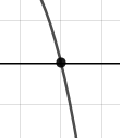
\includegraphics[width = 0.3\textwidth]{../Figures/polyZeroBehaviorAB.png}\item 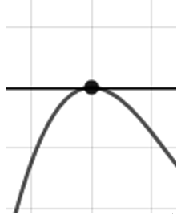
\includegraphics[width = 0.3\textwidth]{../Figures/polyZeroBehaviorBB.png}\item 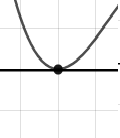
\includegraphics[width = 0.3\textwidth]{../Figures/polyZeroBehaviorCB.png}\item 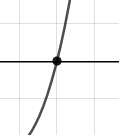
\includegraphics[width = 0.3\textwidth]{../Figures/polyZeroBehaviorDB.png}\end{multicols}\item None of the above.
\end{enumerate} }
\litem{
Construct the lowest-degree polynomial given the zeros below. Then, choose the intervals that contain the coefficients of the polynomial in the form $x^3+bx^2+cx+d$.\[ -3 + 2 i \text{ and } -4 \]\begin{enumerate}[label=\Alph*.]
\item \( b \in [10, 19], c \in [32, 39], \text{ and } d \in [51, 63] \)
\item \( b \in [-1, 3], c \in [4, 8], \text{ and } d \in [11, 17] \)
\item \( b \in [-1, 3], c \in [-4, 3], \text{ and } d \in [-12, -5] \)
\item \( b \in [-11, -7], c \in [32, 39], \text{ and } d \in [-52, -50] \)
\item \( \text{None of the above.} \)

\end{enumerate} }
\litem{
Construct the lowest-degree polynomial given the zeros below. Then, choose the intervals that contain the coefficients of the polynomial in the form $ax^3+bx^2+cx+d$.\[ \frac{7}{5}, \frac{-5}{2}, \text{ and } \frac{1}{2} \]\begin{enumerate}[label=\Alph*.]
\item \( a \in [18, 21], b \in [65, 73], c \in [23, 32], \text{ and } d \in [-35, -33] \)
\item \( a \in [18, 21], b \in [8, 17], c \in [-95, -77], \text{ and } d \in [33, 37] \)
\item \( a \in [18, 21], b \in [8, 17], c \in [-95, -77], \text{ and } d \in [-35, -33] \)
\item \( a \in [18, 21], b \in [-33, -27], c \in [-68, -57], \text{ and } d \in [33, 37] \)
\item \( a \in [18, 21], b \in [-18, -3], c \in [-95, -77], \text{ and } d \in [-35, -33] \)

\end{enumerate} }
\litem{
Which of the following equations \textit{could} be of the graph presented below?
\begin{center}
    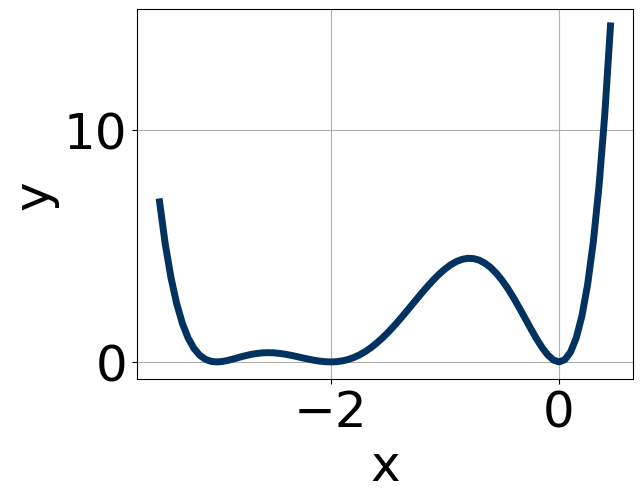
\includegraphics[width=0.5\textwidth]{../Figures/polyGraphToFunctionB.png}
\end{center}
\begin{enumerate}[label=\Alph*.]
\item \( 14x^{11} (x + 3)^{6} (x + 2)^{7} \)
\item \( 16x^{10} (x + 3)^{4} (x + 2)^{11} \)
\item \( -4x^{8} (x + 3)^{8} (x + 2)^{4} \)
\item \( 8x^{6} (x + 3)^{10} (x + 2)^{10} \)
\item \( -5x^{8} (x + 3)^{6} (x + 2)^{7} \)

\end{enumerate} }
\litem{
Describe the zero behavior of the zero $x = 9$ of the polynomial below.\[ f(x) = -3(x + 9)^{6}(x - 9)^{11}(x - 5)^{8}(x + 5)^{9} \]\begin{enumerate}[label=\Alph*.]
\begin{multicols}{2}\item 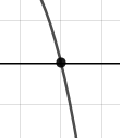
\includegraphics[width = 0.3\textwidth]{../Figures/polyZeroBehaviorCopyAB.png}\item 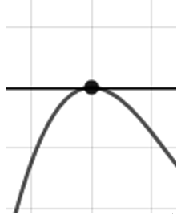
\includegraphics[width = 0.3\textwidth]{../Figures/polyZeroBehaviorCopyBB.png}\item 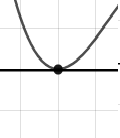
\includegraphics[width = 0.3\textwidth]{../Figures/polyZeroBehaviorCopyCB.png}\item 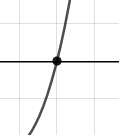
\includegraphics[width = 0.3\textwidth]{../Figures/polyZeroBehaviorCopyDB.png}\end{multicols}\item None of the above.
\end{enumerate} }
\litem{
Construct the lowest-degree polynomial given the zeros below. Then, choose the intervals that contain the coefficients of the polynomial in the form $ax^3+bx^2+cx+d$.\[ \frac{-5}{2}, \frac{4}{3}, \text{ and } -1 \]\begin{enumerate}[label=\Alph*.]
\item \( a \in [1, 10], b \in [13, 15], c \in [-15, -4], \text{ and } d \in [10, 26] \)
\item \( a \in [1, 10], b \in [-2, 5], c \in [-31, -24], \text{ and } d \in [-22, -12] \)
\item \( a \in [1, 10], b \in [-14, -11], c \in [-15, -4], \text{ and } d \in [10, 26] \)
\item \( a \in [1, 10], b \in [13, 15], c \in [-15, -4], \text{ and } d \in [-22, -12] \)
\item \( a \in [1, 10], b \in [-19, -15], c \in [-3, -2], \text{ and } d \in [10, 26] \)

\end{enumerate} }
\litem{
Describe the end behavior of the polynomial below.\[ f(x) = 2(x - 3)^{5}(x + 3)^{10}(x + 7)^{4}(x - 7)^{5} \]\begin{enumerate}[label=\Alph*.]
\begin{multicols}{2}\item 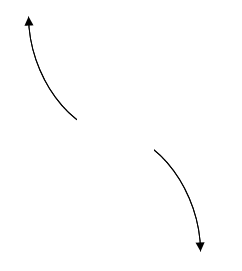
\includegraphics[width = 0.3\textwidth]{../Figures/polyEndBehaviorCopyAC.png}\item 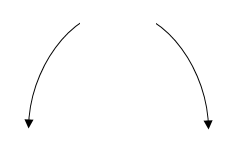
\includegraphics[width = 0.3\textwidth]{../Figures/polyEndBehaviorCopyBC.png}\item 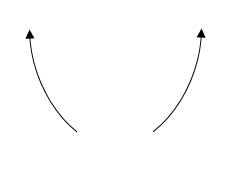
\includegraphics[width = 0.3\textwidth]{../Figures/polyEndBehaviorCopyCC.png}\item 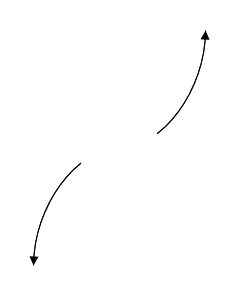
\includegraphics[width = 0.3\textwidth]{../Figures/polyEndBehaviorCopyDC.png}\end{multicols}\item None of the above.
\end{enumerate} }
\litem{
Construct the lowest-degree polynomial given the zeros below. Then, choose the intervals that contain the coefficients of the polynomial in the form $x^3+bx^2+cx+d$.\[ -3 - 5 i \text{ and } -4 \]\begin{enumerate}[label=\Alph*.]
\item \( b \in [-11, -8], c \in [57.4, 58.57], \text{ and } d \in [-141, -128] \)
\item \( b \in [1, 5], c \in [8.96, 9.07], \text{ and } d \in [16, 25] \)
\item \( b \in [9, 15], c \in [57.4, 58.57], \text{ and } d \in [136, 145] \)
\item \( b \in [1, 5], c \in [6.8, 8.11], \text{ and } d \in [12, 18] \)
\item \( \text{None of the above.} \)

\end{enumerate} }
\litem{
Describe the end behavior of the polynomial below.\[ f(x) = -2(x - 8)^{4}(x + 8)^{5}(x + 4)^{2}(x - 4)^{2} \]\begin{enumerate}[label=\Alph*.]
\begin{multicols}{2}\item 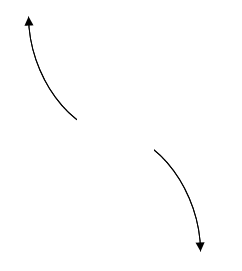
\includegraphics[width = 0.3\textwidth]{../Figures/polyEndBehaviorAC.png}\item 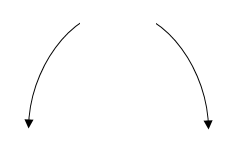
\includegraphics[width = 0.3\textwidth]{../Figures/polyEndBehaviorBC.png}\item 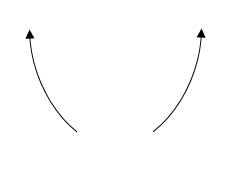
\includegraphics[width = 0.3\textwidth]{../Figures/polyEndBehaviorCC.png}\item 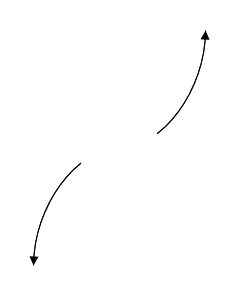
\includegraphics[width = 0.3\textwidth]{../Figures/polyEndBehaviorDC.png}\end{multicols}\item None of the above.
\end{enumerate} }
\litem{
Which of the following equations \textit{could} be of the graph presented below?
\begin{center}
    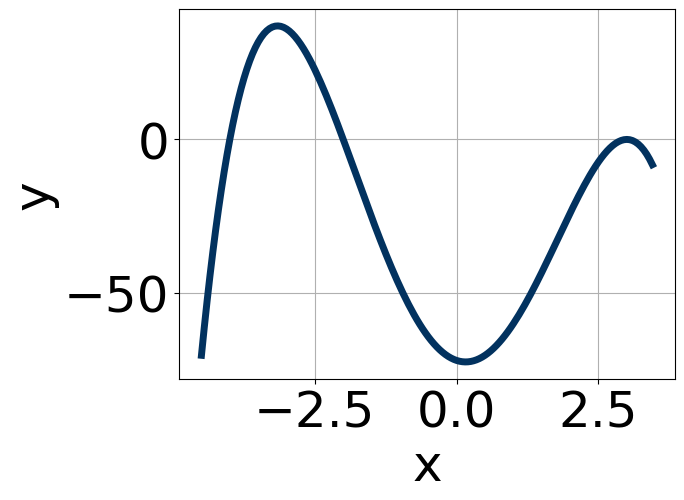
\includegraphics[width=0.5\textwidth]{../Figures/polyGraphToFunctionCopyC.png}
\end{center}
\begin{enumerate}[label=\Alph*.]
\item \( -2(x - 3)^{6} (x + 4)^{10} (x + 2)^{5} \)
\item \( 6(x - 3)^{10} (x + 4)^{11} (x + 2)^{7} \)
\item \( 19(x - 3)^{6} (x + 4)^{9} (x + 2)^{10} \)
\item \( -19(x - 3)^{9} (x + 4)^{6} (x + 2)^{11} \)
\item \( -14(x - 3)^{8} (x + 4)^{11} (x + 2)^{5} \)

\end{enumerate} }
\litem{
Describe the zero behavior of the zero $x = 9$ of the polynomial below.\[ f(x) = 2(x + 5)^{4}(x - 5)^{2}(x + 9)^{11}(x - 9)^{8} \]\begin{enumerate}[label=\Alph*.]
\begin{multicols}{2}\item 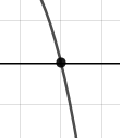
\includegraphics[width = 0.3\textwidth]{../Figures/polyZeroBehaviorAC.png}\item 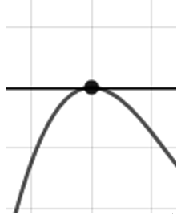
\includegraphics[width = 0.3\textwidth]{../Figures/polyZeroBehaviorBC.png}\item 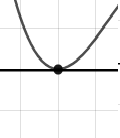
\includegraphics[width = 0.3\textwidth]{../Figures/polyZeroBehaviorCC.png}\item 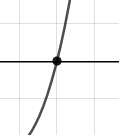
\includegraphics[width = 0.3\textwidth]{../Figures/polyZeroBehaviorDC.png}\end{multicols}\item None of the above.
\end{enumerate} }
\litem{
Construct the lowest-degree polynomial given the zeros below. Then, choose the intervals that contain the coefficients of the polynomial in the form $x^3+bx^2+cx+d$.\[ 5 + 3 i \text{ and } -2 \]\begin{enumerate}[label=\Alph*.]
\item \( b \in [-3, 4], c \in [-1, 3], \text{ and } d \in [-8, -3] \)
\item \( b \in [5, 14], c \in [7, 19], \text{ and } d \in [-75, -65] \)
\item \( b \in [-3, 4], c \in [-7, -2], \text{ and } d \in [-10, -8] \)
\item \( b \in [-12, -7], c \in [7, 19], \text{ and } d \in [67, 75] \)
\item \( \text{None of the above.} \)

\end{enumerate} }
\litem{
Construct the lowest-degree polynomial given the zeros below. Then, choose the intervals that contain the coefficients of the polynomial in the form $ax^3+bx^2+cx+d$.\[ \frac{-2}{3}, \frac{7}{3}, \text{ and } 6 \]\begin{enumerate}[label=\Alph*.]
\item \( a \in [3, 10], b \in [-71, -67], c \in [69, 84], \text{ and } d \in [82, 94] \)
\item \( a \in [3, 10], b \in [-71, -67], c \in [69, 84], \text{ and } d \in [-86, -79] \)
\item \( a \in [3, 10], b \in [66, 74], c \in [69, 84], \text{ and } d \in [-86, -79] \)
\item \( a \in [3, 10], b \in [-43, -34], c \in [-106, -100], \text{ and } d \in [82, 94] \)
\item \( a \in [3, 10], b \in [-81, -79], c \in [175, 180], \text{ and } d \in [-86, -79] \)

\end{enumerate} }
\litem{
Which of the following equations \textit{could} be of the graph presented below?
\begin{center}
    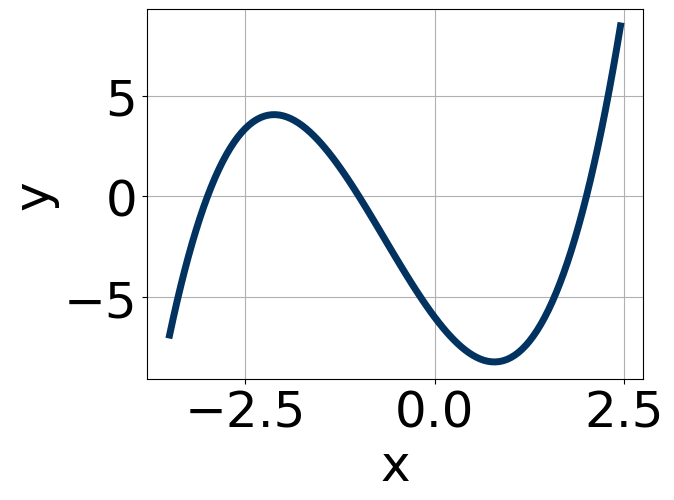
\includegraphics[width=0.5\textwidth]{../Figures/polyGraphToFunctionC.png}
\end{center}
\begin{enumerate}[label=\Alph*.]
\item \( 12(x - 2)^{6} (x + 3)^{5} (x + 1)^{7} \)
\item \( 20(x - 2)^{7} (x + 3)^{5} (x + 1)^{9} \)
\item \( -17(x - 2)^{4} (x + 3)^{7} (x + 1)^{5} \)
\item \( -14(x - 2)^{7} (x + 3)^{11} (x + 1)^{7} \)
\item \( 9(x - 2)^{4} (x + 3)^{6} (x + 1)^{9} \)

\end{enumerate} }
\litem{
Describe the zero behavior of the zero $x = 4$ of the polynomial below.\[ f(x) = 5(x - 4)^{9}(x + 4)^{10}(x - 7)^{9}(x + 7)^{10} \]\begin{enumerate}[label=\Alph*.]
\begin{multicols}{2}\item \includegraphics[width = 0.3\textwidth]{../Figures/polyZeroBehaviorCopyAC.png}\item \includegraphics[width = 0.3\textwidth]{../Figures/polyZeroBehaviorCopyBC.png}\item \includegraphics[width = 0.3\textwidth]{../Figures/polyZeroBehaviorCopyCC.png}\item \includegraphics[width = 0.3\textwidth]{../Figures/polyZeroBehaviorCopyDC.png}\end{multicols}\item None of the above.
\end{enumerate} }
\end{enumerate}

\end{document}